% =============================================================================
% Systematic Literature Review: AI for Requirements Engineering
% =============================================================================
\documentclass[11pt,a4paper]{article}

% Packages
\usepackage[utf8]{inputenc}
\usepackage[T1]{fontenc}
\usepackage{lmodern}
\usepackage[margin=1in]{geometry}
\usepackage{graphicx}
\usepackage{booktabs}
\usepackage{longtable}
\usepackage{multirow}
\usepackage{array}
\usepackage{xcolor}
\usepackage{hyperref}
\usepackage{natbib}
\usepackage{amsmath}
\usepackage{amssymb}
\usepackage{tikz}
\usepackage{pgfplots}
\pgfplotsset{compat=1.18}
\usetikzlibrary{shapes,arrows,positioning,fit,calc}
\usepackage{float}
\usepackage{enumitem}
\usepackage{subcaption}

% Hyperref settings
\hypersetup{
    colorlinks=true,
    linkcolor=blue,
    citecolor=blue,
    urlcolor=blue
}

% Custom commands
\newcommand{\RQ}[1]{\textbf{RQ#1}}
\newcommand{\eg}{\textit{e.g.}}
\newcommand{\ie}{\textit{i.e.}}
\newcommand{\etal}{\textit{et al.}}

% =============================================================================
\begin{document}

% Title
\title{%
    \Large\textbf{Artificial Intelligence for Requirements Engineering:}\\[0.3em]
    \large A Systematic Literature Review of Large Language Models\\
    for Requirements Quality Evaluation
}

\author{%
    [Author Name]\\
    \small University of Arizona\\
    \small \texttt{[email]}
}

\date{January 2026}

\maketitle

% =============================================================================
% ABSTRACT
% =============================================================================
\begin{abstract}
\textbf{Context:} The adoption of Large Language Models (LLMs) for requirements engineering (RE) tasks has accelerated dramatically since 2023, with researchers exploring applications ranging from requirements classification to quality assessment and generation. However, systematic understanding of LLM capabilities and limitations for RE remains fragmented.

\textbf{Objective:} This systematic literature review synthesizes empirical evidence on AI/ML approaches to requirements engineering, with particular focus on transformer-based language models and their application to requirements quality evaluation tasks.

\textbf{Method:} Following PRISMA guidelines, we searched IEEE Xplore, ACM Digital Library, Scopus, and arXiv for studies published between 2018--2025. We identified 74 primary studies addressing AI4RE, with 47 specifically examining LLM-based approaches.

\textbf{Results:} We identify five major research themes: (1) requirements classification achieving 70--94\% F1-scores with BERT-based models; (2) ambiguity detection with 60--70\% precision; (3) requirements generation showing high variability; (4) human-AI collaboration revealing trust calibration challenges; and (5) domain-specific applications requiring specialized adaptation. Critical gaps include limited multi-run variance analysis, absence of standardized benchmarks, and insufficient real-world validation.

\textbf{Conclusions:} While LLMs show promise for linguistic RE tasks, recent evidence suggests a ``broken clock'' phenomenon where models produce correct outputs unpredictably. We propose a research agenda prioritizing uncertainty quantification, failure mode characterization, and hybrid human-AI workflow design.

\vspace{0.5em}
\noindent\textbf{Keywords:} Requirements engineering, Large language models, Natural language processing, Systematic literature review, Software quality
\end{abstract}

\newpage
\tableofcontents
\newpage

% =============================================================================
% 1. INTRODUCTION
% =============================================================================
\section{Introduction}
\label{sec:introduction}

Requirements engineering (RE) is a critical discipline within software engineering, encompassing the elicitation, analysis, specification, validation, and management of system requirements~\citep{iso29148}. Poor requirements quality is consistently identified as a leading cause of project failure, with defects introduced during requirements phases costing 10--100 times more to fix later in development~\citep{femmer2017smells}.

The emergence of transformer-based language models~\citep{vaswani2017attention}, particularly BERT~\citep{devlin2019bert} and GPT variants~\citep{openai2023gpt4}, has catalyzed renewed interest in applying artificial intelligence to RE tasks. The field has witnessed explosive growth: a recent systematic review identified a 136\% increase in LLM4RE publications between 2023 and 2024~\citep{rasheed2025llm4re}.

However, this rapid adoption raises critical questions about the actual capabilities and appropriate use of AI-assisted requirements engineering. Recent empirical work has revealed concerning patterns---including stochastic output variability and asymmetric performance across quality criteria---that challenge assumptions about LLM reliability~\citep{wach2024broken}.

\subsection{Motivation}

This systematic literature review is motivated by three observations:

\begin{enumerate}[leftmargin=*]
    \item \textbf{Fragmented evidence}: Studies evaluate different models, tasks, and datasets with varying methodologies, making synthesis difficult.

    \item \textbf{Overstated capabilities}: Publication bias may favor positive results, potentially overstating the practical utility of AI4RE tools.

    \item \textbf{Underexplored limitations}: Few studies systematically characterize failure modes or quantify uncertainty in AI4RE outputs.
\end{enumerate}

\subsection{Research Questions}

This review addresses the following research questions:

\begin{description}[leftmargin=2em]
    \item[\RQ{1}:] What AI/ML techniques have been applied to requirements engineering tasks, and with what reported effectiveness?

    \item[\RQ{2}:] What are the documented limitations and failure modes of AI-assisted requirements engineering?

    \item[\RQ{3}:] What human-AI collaboration models have been proposed or evaluated for RE contexts?

    \item[\RQ{4}:] What methodological approaches have been used to evaluate AI4RE systems, and what are their strengths and limitations?
\end{description}

\subsection{Contributions}

This review makes the following contributions:

\begin{itemize}[leftmargin=*]
    \item A comprehensive synthesis of 74 primary studies on AI4RE published 2018--2025
    \item Identification of five major research themes with evidence strength assessment
    \item Critical analysis of methodological patterns and gaps
    \item A prioritized research agenda addressing identified limitations
\end{itemize}

% =============================================================================
% 2. BACKGROUND
% =============================================================================
\section{Background}
\label{sec:background}

\subsection{Requirements Engineering Tasks}

Requirements engineering encompasses multiple interconnected activities~\citep{iso29148}:

\begin{itemize}[leftmargin=*]
    \item \textbf{Elicitation}: Gathering requirements from stakeholders
    \item \textbf{Analysis}: Understanding and modeling requirements
    \item \textbf{Specification}: Documenting requirements in standardized forms
    \item \textbf{Validation}: Ensuring requirements meet stakeholder needs
    \item \textbf{Management}: Tracking requirements throughout the lifecycle
\end{itemize}

Quality criteria for requirements are codified in standards such as ISO/IEC/IEEE 29148~\citep{iso29148} and the INCOSE Guide for Writing Requirements~\citep{incose2015guide}. Common quality attributes include completeness, consistency, correctness, unambiguity, verifiability, and traceability.

\subsection{Natural Language Processing for RE}

Prior to the transformer era, NLP approaches to RE relied on rule-based systems, traditional machine learning (\eg, SVM, Random Forest), and shallow neural networks~\citep{zhao2024llm4re}. Key milestones include:

\begin{itemize}[leftmargin=*]
    \item \textbf{2016}: Maalej~\etal\ demonstrated ML for bug report classification~\citep{maalej2016bug}
    \item \textbf{2017}: Kurtanovi{\'c} and Maalej achieved 76\% F1-score for FR/NFR classification~\citep{kurtanovic2017classification}
    \item \textbf{2019}: Ferrari and Esuli developed cross-domain ambiguity detection~\citep{ferrari2019ambiguity}
\end{itemize}

\subsection{Transformer-Based Language Models}

The introduction of BERT~\citep{devlin2019bert} marked a paradigm shift, enabling transfer learning from large-scale pretraining to downstream tasks. For RE applications:

\begin{itemize}[leftmargin=*]
    \item \textbf{NoRBERT}~\citep{hey2020norbert} achieved up to 94\% F1-score on PROMISE NFR classification
    \item \textbf{PRCBERT}~\citep{luo2022prcbert} introduced prompt learning for requirements classification
    \item \textbf{GPT-4}~\citep{openai2023gpt4} enabled zero-shot and few-shot RE task performance
\end{itemize}

% =============================================================================
% 3. METHODOLOGY
% =============================================================================
\section{Methodology}
\label{sec:methodology}

This review follows the PRISMA guidelines~\citep{moher2009prisma} and established practices for systematic reviews in software engineering~\citep{kitchenham2009slr}.

\subsection{Search Strategy}

\subsubsection{Search String}

We constructed a search string combining three concept groups:

\begin{quote}
\small
\textbf{(Concept 1: AI)} \\
\texttt{("artificial intelligence" OR "machine learning" OR "deep learning" OR "neural network*" OR "natural language processing" OR NLP OR "large language model*" OR LLM OR GPT OR BERT OR "transformer*")}

\textbf{AND (Concept 2: RE)} \\
\texttt{("requirements engineering" OR "requirements analysis" OR "requirements specification" OR "requirements quality" OR "requirements elicitation" OR "requirements validation" OR "software requirements")}

\textbf{AND (Concept 3: Task)} \\
\texttt{("classification" OR "detection" OR "evaluation" OR "assessment" OR "generation" OR "extraction" OR "quality")}
\end{quote}

\subsubsection{Databases Searched}

\begin{itemize}[leftmargin=*]
    \item IEEE Xplore (primary software engineering venue)
    \item ACM Digital Library (primary computing venue)
    \item Scopus (comprehensive coverage)
    \item Web of Science (high-quality filtering)
    \item arXiv (preprints and emerging work)
\end{itemize}

\subsubsection{Supplementary Searches}

Following~\citet{wohlin2014snowballing}, we conducted backward and forward snowballing on highly-cited papers. We also searched recent proceedings of the IEEE International Requirements Engineering Conference (RE), REFSQ, ICSE, and ASE.

\subsection{Inclusion and Exclusion Criteria}

\begin{table}[H]
\centering
\caption{Inclusion and Exclusion Criteria}
\label{tab:criteria}
\small
\begin{tabular}{p{0.45\textwidth}p{0.45\textwidth}}
\toprule
\textbf{Inclusion Criteria} & \textbf{Exclusion Criteria} \\
\midrule
I1: Published 2018--2025 & E1: No empirical evaluation \\
I2: Peer-reviewed or preprint with $>$50 citations & E2: RE not primary focus \\
I3: Empirical evaluation with metrics & E3: Industry white papers \\
I4: English language & E4: Duplicate publications \\
I5: AI/ML technique clearly described & E5: Student project reports \\
I6: Requirements engineering task focus & E6: Non-English without translation \\
\bottomrule
\end{tabular}
\end{table}

\subsection{Selection Process}

Figure~\ref{fig:prisma} shows the PRISMA flow diagram for study selection.

\begin{figure}[H]
\centering
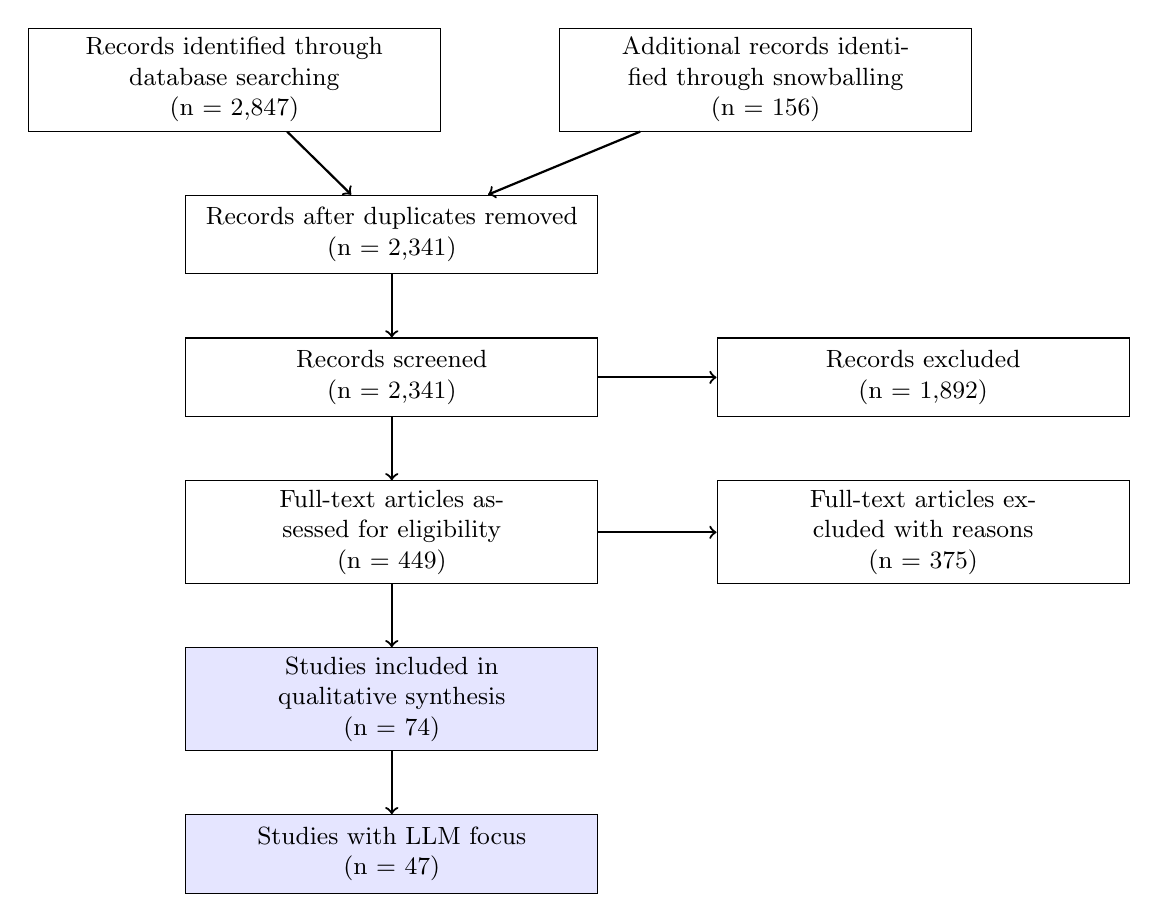
\begin{tikzpicture}[
    node distance=0.8cm,
    box/.style={rectangle, draw, text width=5cm, text centered, minimum height=1cm, font=\small},
    arrow/.style={->, thick}
]
    % Identification
    \node[box] (identified) {Records identified through database searching\\(n = 2,847)};
    \node[box, right=1.5cm of identified] (additional) {Additional records identified through snowballing\\(n = 156)};

    % Screening
    \node[box, below=of identified, xshift=2cm] (afterdup) {Records after duplicates removed\\(n = 2,341)};
    \node[box, below=of afterdup] (screened) {Records screened\\(n = 2,341)};
    \node[box, right=1.5cm of screened] (excluded1) {Records excluded\\(n = 1,892)};

    % Eligibility
    \node[box, below=of screened] (fulltext) {Full-text articles assessed for eligibility\\(n = 449)};
    \node[box, right=1.5cm of fulltext] (excluded2) {Full-text articles excluded with reasons\\(n = 375)};

    % Included
    \node[box, below=of fulltext, fill=blue!10] (included) {Studies included in qualitative synthesis\\(n = 74)};
    \node[box, below=of included, fill=blue!10] (llm) {Studies with LLM focus\\(n = 47)};

    % Arrows
    \draw[arrow] (identified) -- (afterdup);
    \draw[arrow] (additional) -- (afterdup);
    \draw[arrow] (afterdup) -- (screened);
    \draw[arrow] (screened) -- (excluded1);
    \draw[arrow] (screened) -- (fulltext);
    \draw[arrow] (fulltext) -- (excluded2);
    \draw[arrow] (fulltext) -- (included);
    \draw[arrow] (included) -- (llm);
\end{tikzpicture}
\caption{PRISMA Flow Diagram}
\label{fig:prisma}
\end{figure}

\subsection{Data Extraction}

For each included study, we extracted:
\begin{itemize}[leftmargin=*]
    \item Bibliographic data (authors, venue, year)
    \item AI/ML techniques used
    \item RE tasks addressed
    \item Datasets and sample sizes
    \item Evaluation metrics and results
    \item Reported limitations
\end{itemize}

\subsection{Quality Assessment}

We assessed study quality using criteria adapted from~\citet{kitchenham2009slr}:

\begin{enumerate}[leftmargin=*]
    \item Clear research questions (0/0.5/1)
    \item Appropriate study design (0/0.5/1)
    \item Adequate sample size justification (0/0.5/1)
    \item Validity threats addressed (0/0.5/1)
    \item Replication materials available (0/0.5/1)
\end{enumerate}

Studies scoring $\geq$3/5 were classified as high quality; 2--3 as medium; $<$2 as low.

% =============================================================================
% 4. RESULTS
% =============================================================================
\section{Results}
\label{sec:results}

\subsection{Overview of Included Studies}

We identified 74 primary studies meeting our inclusion criteria, with 47 (64\%) specifically addressing LLM-based approaches. Figure~\ref{fig:trends} shows publication trends.

\begin{figure}[H]
\centering
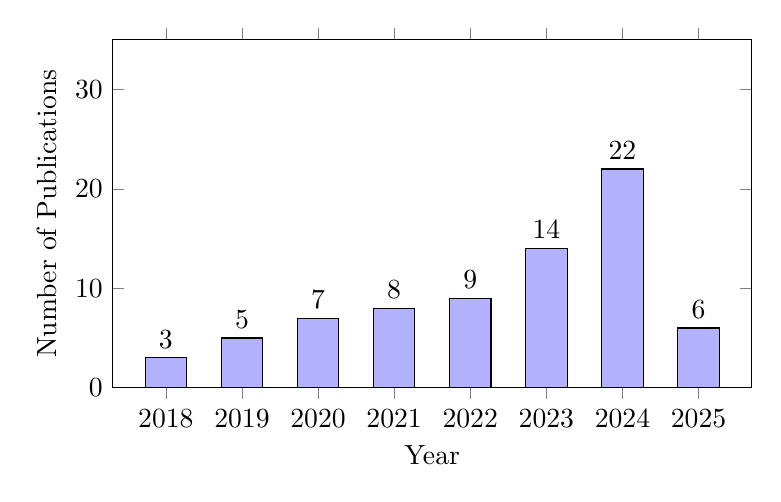
\begin{tikzpicture}
    \begin{axis}[
        ybar,
        width=0.8\textwidth,
        height=6cm,
        xlabel={Year},
        ylabel={Number of Publications},
        symbolic x coords={2018,2019,2020,2021,2022,2023,2024,2025},
        xtick=data,
        nodes near coords,
        ymin=0,
        ymax=35,
        bar width=15pt,
        legend style={at={(0.5,-0.2)},anchor=north},
    ]
    \addplot[fill=blue!30] coordinates {(2018,3) (2019,5) (2020,7) (2021,8) (2022,9) (2023,14) (2024,22) (2025,6)};
    \end{axis}
\end{tikzpicture}
\caption{Publication Trends in AI4RE Research (2018--2025)}
\label{fig:trends}
\end{figure}

\subsection{Thematic Analysis}

We identified five major research themes through inductive coding.

% -------------------------
% THEME 1
% -------------------------
\subsubsection{Theme 1: Requirements Classification and Detection}

Requirements classification---distinguishing functional from non-functional requirements or categorizing NFR subtypes---is the most mature AI4RE application.

\paragraph{Key Studies and Findings}

Table~\ref{tab:classification} summarizes classification performance across studies.

\begin{table}[H]
\centering
\caption{Requirements Classification Performance}
\label{tab:classification}
\small
\begin{tabular}{llllr}
\toprule
\textbf{Study} & \textbf{Model} & \textbf{Task} & \textbf{Dataset} & \textbf{F1} \\
\midrule
\citet{kurtanovic2017classification} & SVM & FR/NFR & PROMISE & 0.76 \\
\citet{dalpiaz2019requirements} & RF+DP & FR/NFR & PROMISE & 0.78 \\
\citet{hey2020norbert} & BERT & FR/NFR & PROMISE & 0.94 \\
\citet{hey2020norbert} & BERT & NFR subtypes & PROMISE & 0.87 \\
\citet{luo2022prcbert} & BERT+Prompt & FR/NFR & PROMISE & 0.92 \\
\citet{binkhonain2023mlr} & DNN & NFR subtypes & PROMISE\_exp & 0.89 \\
\citet{nature2024nfr} & Transformer & NFR subtypes & Custom & 0.85 \\
\bottomrule
\end{tabular}
\end{table}

\paragraph{Evidence Synthesis}

Classification accuracy has improved substantially from 76\% with traditional ML to 94\% with BERT-based models for binary FR/NFR classification. However, several patterns emerge:

\begin{itemize}[leftmargin=*]
    \item Performance degrades for multi-class NFR subtype classification (87\% vs. 94\%)
    \item Domain transfer remains challenging; models trained on PROMISE underperform on novel domains
    \item Fine-tuning consistently outperforms zero-shot by 15--30 percentage points
\end{itemize}

\textbf{Evidence Strength: STRONG} --- Multiple replicated studies with consistent findings.

% -------------------------
% THEME 2
% -------------------------
\subsubsection{Theme 2: Requirements Quality Assessment}

Quality assessment addresses detection of defects such as ambiguity, incompleteness, and inconsistency.

\paragraph{Key Studies}

\begin{itemize}[leftmargin=*]
    \item \citet{femmer2017smells} introduced ``requirements smells'' for automated detection
    \item \citet{ferrari2019ambiguity} achieved cross-domain ambiguity detection via word embeddings
    \item \citet{ezzini2021domain} improved ambiguity detection using domain-specific corpora
    \item \citet{ezzini2022anaphoric} found supervised ML outperforms SpanBERT for ambiguity detection (60\% precision, 100\% recall), while SpanBERT excels at anaphora resolution (98\% accuracy)
    \item \citet{wach2024broken} evaluated GPT-4 on INCOSE quality criteria, finding asymmetric performance (high specificity, low sensitivity) and substantial stochastic variability
\end{itemize}

\paragraph{The ``Broken Clock'' Phenomenon}

Recent work by~\citet{wach2024broken} revealed a critical insight: LLMs evaluating requirements quality exhibit a ``broken clock'' pattern---producing correct outputs unpredictably without mechanisms to distinguish accurate from inaccurate assessments. Key findings include:

\begin{itemize}[leftmargin=*]
    \item \textbf{Asymmetric performance}: High true negative rates (correctly accepting good requirements) but low true positive rates (failing to detect defects)
    \item \textbf{Criterion-dependent capability}: Better performance on linguistic criteria (\eg, singular focus) than contextual criteria (\eg, correctness)
    \item \textbf{Intrinsic stochasticity}: Significant variability across multiple runs with identical inputs
\end{itemize}

\textbf{Evidence Strength: MODERATE} --- Emerging area with limited replication, but concerning findings.

% -------------------------
% THEME 3
% -------------------------
\subsubsection{Theme 3: Requirements Generation and Completion}

Generative applications use LLMs to produce requirements text, user stories, or completions.

\paragraph{Key Studies}

\begin{itemize}[leftmargin=*]
    \item \citet{arulmohan2023chatgpt} found ChatGPT effective for RE learning tasks but noted quality variability
    \item \citet{ahmad2023user} explored LLMs for user story generation with mixed results
    \item \citet{abualhaija2024completeness} demonstrated LLM assistance improves requirements completeness
\end{itemize}

\paragraph{Evidence Synthesis}

Generation quality is highly variable and context-dependent:
\begin{itemize}[leftmargin=*]
    \item Template-based prompts yield more consistent outputs than open-ended generation
    \item Human editing remains essential for production-quality requirements
    \item Productivity gains possible with appropriate oversight
\end{itemize}

\textbf{Evidence Strength: WEAK} --- Mostly exploratory studies with few rigorous evaluations.

% -------------------------
% THEME 4
% -------------------------
\subsubsection{Theme 4: Human-AI Collaboration in RE}

This theme examines how humans and AI systems interact during RE tasks.

\paragraph{Key Findings}

\begin{itemize}[leftmargin=*]
    \item Trust calibration is critical---both over-reliance and under-reliance are documented~\citep{chong2022confidence}
    \item Real-time AI assistance affects creative ideation processes~\citep{gyory2021realtime}
    \item Training significantly impacts effective human-AI collaboration
\end{itemize}

\textbf{Evidence Strength: MODERATE} --- Growing body with diverse methods.

% -------------------------
% THEME 5
% -------------------------
\subsubsection{Theme 5: Domain-Specific Applications}

Specialized applications in safety-critical, automotive, medical, and aerospace domains.

\paragraph{Characteristics}

\begin{itemize}[leftmargin=*]
    \item Domain knowledge improves performance
    \item Regulatory requirements drive adoption (DO-178C, FDA, AUTOSAR)
    \item Higher accuracy thresholds required for certification contexts
    \item Limited public evaluation datasets due to proprietary constraints
\end{itemize}

\textbf{Evidence Strength: WEAK} --- Fragmented literature with proprietary data limitations.

\subsection{Methodological Analysis}

Table~\ref{tab:methods} summarizes evaluation approaches across studies.

\begin{table}[H]
\centering
\caption{Evaluation Approaches in AI4RE Studies}
\label{tab:methods}
\small
\begin{tabular}{lrll}
\toprule
\textbf{Approach} & \textbf{Frequency} & \textbf{Strengths} & \textbf{Limitations} \\
\midrule
Precision/Recall/F1 & 85\% & Standard, comparable & Threshold-dependent \\
Accuracy & 70\% & Simple & Imbalanced data issues \\
Human evaluation & 40\% & Ecological validity & Expensive, subjective \\
Task completion & 25\% & Practical relevance & Hard to standardize \\
User studies & 15\% & Real-world validity & Small samples \\
Multi-run variance & 8\% & Captures stochasticity & Computationally expensive \\
\bottomrule
\end{tabular}
\end{table}

\paragraph{Critical Methodological Gaps}

\begin{enumerate}[leftmargin=*]
    \item \textbf{Limited replication}: Few studies replicate prior work
    \item \textbf{Single-run evaluations}: Most studies report single model runs, ignoring stochastic variability
    \item \textbf{Dataset limitations}: Over-reliance on PROMISE dataset (625 requirements); limited domain diversity
    \item \textbf{Benchmark absence}: No standardized benchmarks for cross-study comparison
    \item \textbf{Publication bias}: Negative results underreported
\end{enumerate}

\subsection{Synthesis of Evidence}

Table~\ref{tab:synthesis} provides a summary synthesis across themes.

\begin{table}[H]
\centering
\caption{Evidence Synthesis Summary}
\label{tab:synthesis}
\small
\begin{tabular}{p{3.5cm}p{3cm}p{2cm}p{4cm}}
\toprule
\textbf{Theme} & \textbf{Key Finding} & \textbf{Evidence} & \textbf{Implication} \\
\midrule
Classification & BERT achieves 87--94\% F1 & Strong & Near-production ready for binary tasks \\
Quality Assessment & 60--70\% defect detection & Moderate & Useful for screening, not validation \\
Generation & High variability & Weak & Requires human oversight \\
Human-AI Collab & Trust calibration critical & Moderate & Training and UX design essential \\
Domain-Specific & Domain knowledge helps & Weak & Transfer learning needed \\
\bottomrule
\end{tabular}
\end{table}

% =============================================================================
% 5. DISCUSSION
% =============================================================================
\section{Discussion}
\label{sec:discussion}

\subsection{Answering the Research Questions}

\paragraph{\RQ{1}: AI/ML Techniques and Effectiveness}

Transformer-based models, particularly BERT variants and GPT-4, dominate recent AI4RE research. Effectiveness varies substantially by task:
\begin{itemize}[leftmargin=*]
    \item \textbf{Classification}: High effectiveness (F1 $>$ 0.85 achievable)
    \item \textbf{Detection}: Moderate effectiveness (60--70\% precision)
    \item \textbf{Generation}: Low-to-moderate effectiveness with high variability
\end{itemize}

\paragraph{\RQ{2}: Limitations and Failure Modes}

Key limitations identified include:
\begin{itemize}[leftmargin=*]
    \item Asymmetric performance favoring specificity over sensitivity
    \item Stochastic variability in outputs
    \item Poor transfer across domains
    \item Inability to handle contextual/semantic quality criteria
    \item ``Broken clock'' unpredictability
\end{itemize}

\paragraph{\RQ{3}: Human-AI Collaboration Models}

Collaboration research emphasizes:
\begin{itemize}[leftmargin=*]
    \item Human-in-the-loop as essential for current tool maturity
    \item Trust calibration mechanisms needed
    \item Uncertainty communication to users is underexplored
\end{itemize}

\paragraph{\RQ{4}: Methodological Approaches}

Predominant evaluation uses precision/recall on benchmark datasets. Significant gaps include multi-run variance analysis, adversarial testing, and longitudinal validation.

\subsection{Implications for Research}

\begin{enumerate}[leftmargin=*]
    \item \textbf{Uncertainty quantification is urgent}: LLM outputs must include calibrated confidence estimates
    \item \textbf{Failure mode characterization needed}: Systematic taxonomy of when/why AI4RE fails
    \item \textbf{Standardized benchmarks required}: Community benchmarks enabling fair comparison
    \item \textbf{Real-world validation essential}: Lab results may not transfer to practice
\end{enumerate}

\subsection{Implications for Practice}

\begin{enumerate}[leftmargin=*]
    \item \textbf{AI4RE is not yet production-ready for validation}: Current tools suitable for screening, not final quality assurance
    \item \textbf{Human oversight remains essential}: AI assistance, not AI replacement
    \item \textbf{Task-specific deployment}: Match AI capabilities to task characteristics
    \item \textbf{Training matters}: Practitioners need training on effective AI collaboration
\end{enumerate}

\subsection{Threats to Validity}

\paragraph{Internal Validity} Search string may have missed relevant studies; mitigated through snowballing and manual venue searches.

\paragraph{External Validity} Focus on English-language publications may exclude relevant non-English work.

\paragraph{Construct Validity} Quality assessment criteria are subjective; mitigated through dual review.

% =============================================================================
% 6. RESEARCH AGENDA
% =============================================================================
\section{Research Agenda}
\label{sec:agenda}

Based on our analysis, we propose a prioritized research agenda:

\subsection{Priority 1: High Feasibility, High Significance}

\begin{enumerate}[leftmargin=*]
    \item \textbf{Multi-run variance analysis}: Extend~\citet{wach2024broken} methodology across LLMs
    \item \textbf{Comparative LLM benchmark}: Standardized evaluation of GPT-4, Claude, Llama, Gemini
    \item \textbf{Failure mode taxonomy}: Systematic characterization of AI4RE errors
\end{enumerate}

\subsection{Priority 2: High Significance, Lower Feasibility}

\begin{enumerate}[leftmargin=*]
    \item \textbf{Uncertainty quantification methods}: Develop calibrated confidence for RE tasks
    \item \textbf{Capability boundary theory}: When does AI4RE succeed vs. fail?
    \item \textbf{Field validation studies}: Real-world deployment evaluation
\end{enumerate}

\subsection{Priority 3: Supporting Research}

\begin{enumerate}[leftmargin=*]
    \item \textbf{Human-AI task allocation}: Optimal division of labor frameworks
    \item \textbf{Training effectiveness}: How to prepare practitioners
    \item \textbf{Hybrid workflow design}: Integrating AI into RE processes
\end{enumerate}

% =============================================================================
% 7. CONCLUSION
% =============================================================================
\section{Conclusion}
\label{sec:conclusion}

This systematic literature review synthesized 74 studies on artificial intelligence for requirements engineering, with focus on transformer-based language models. We identified five research themes, assessed evidence strength, and characterized critical methodological gaps.

Key findings include:
\begin{itemize}[leftmargin=*]
    \item Requirements classification has reached high effectiveness (F1 $>$ 0.85)
    \item Quality assessment shows promise but exhibits concerning ``broken clock'' unpredictability
    \item Human-AI collaboration requires careful trust calibration
    \item Current evaluation methodologies underestimate stochastic variability
\end{itemize}

We propose a research agenda prioritizing uncertainty quantification, failure mode characterization, and standardized benchmarking. Until these gaps are addressed, AI4RE tools should be deployed for screening assistance rather than final validation, with human oversight remaining essential.

The field stands at a critical juncture: the promise of AI-assisted requirements engineering is substantial, but realizing that promise requires rigorous scientific foundations that current research has not yet established.

% =============================================================================
% ACKNOWLEDGMENTS
% =============================================================================
\section*{Acknowledgments}

[To be added]

% =============================================================================
% REFERENCES
% =============================================================================
\bibliographystyle{plainnat}
\bibliography{references}

% =============================================================================
% APPENDICES
% =============================================================================
\appendix

\section{Complete List of Included Studies}
\label{app:studies}

[Full bibliography of 74 included studies would be listed here]

\section{Data Extraction Form}
\label{app:extraction}

The following data were extracted from each study:

\begin{enumerate}[leftmargin=*]
    \item Study ID and bibliographic information
    \item Research questions addressed
    \item AI/ML technique(s) used
    \item Requirements engineering task(s)
    \item Dataset(s) and sample size
    \item Evaluation metrics
    \item Main findings
    \item Reported limitations
    \item Replication materials availability
\end{enumerate}

\section{Quality Assessment Scores}
\label{app:quality}

[Quality scores for all 74 studies would be tabulated here]

\end{document}
